\section{An extension: managing accumulated straddle exposure}\label{sec:19}

Entry sizing and strategy allocation leave a third question: should an existing option position be trimmed as risk accumulates? A separate experiment uses a \$10 million joint whole-contract account, fixed 90\% put / 10\% straddle budgets and half-size entries in both sleeves. It does not replace the bandit accounts or the fractional-index Q experiment above.


A nonnegative regression predicts the magnitude of next-session straddle-book market P\&L from gross straddle vega and the preceding 21-session RMS P\&L. The coefficients and a 75th-percentile risk-per-NAV cutoff use 2018--2021 data. Cuts are inactive then, so this fits the warning without validating the management rule. When the reference-book warning is high, new straddles pause and existing cohorts target half their original integer counts at the next close. Trims remain in place; put rules are unchanged. This is an interpretable risk rule, not a learned Q-management policy.


\begin{figure}[!htbp]\centering
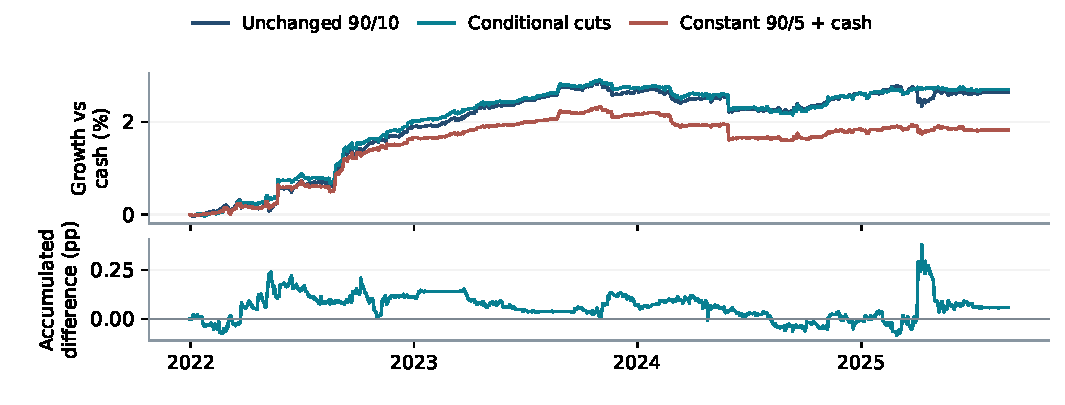
\includegraphics[width=\linewidth]{straddle_management.pdf}
\caption{Separate joint-contract management trial, January 2022--August 2025. Upper panel: compounded growth relative to cash. Lower panel: cumulative daily excess-return difference, conditional cuts minus unchanged 90/10. This is not the Q-index account.}\label{fig:straddle-management}
\end{figure}

\begin{table}[H]\centering\small
\caption{Separate joint-contract management trial, January 2022--August 2025.}
\setlength{\tabcolsep}{4pt}\renewcommand{\arraystretch}{1.18}
\begin{tabularx}{\textwidth}{@{}>{\hsize=1.87500\hsize\linewidth=\hsize\raggedright\arraybackslash}X>{\hsize=0.83008\hsize\linewidth=\hsize\raggedleft\arraybackslash}X>{\hsize=0.78125\hsize\linewidth=\hsize\raggedleft\arraybackslash}X>{\hsize=0.68359\hsize\linewidth=\hsize\raggedleft\arraybackslash}X>{\hsize=0.83008\hsize\linewidth=\hsize\raggedleft\arraybackslash}X@{}}\toprule
\textbf{Account} & \textbf{Mean excess (\%)} & \textbf{Vol. (\%)} & \textbf{Sharpe} & \textbf{Drawdown (\%)}\\\midrule
Unchanged 90/10 & 0.718 & 0.525 & 1.365 & 0.676\\
Conditional cuts & 0.733 & 0.465 & 1.576 & 0.734\\
Constant 90/5 + cash & 0.499 & 0.435 & 1.147 & 0.719\\
\bottomrule\end{tabularx}\end{table}

During January 2022--August 2025, conditional cuts raise excess Sharpe from 1.365 to 1.576, mainly by reducing volatility while preserving the arithmetic mean excess return. Cash-relative maximum drawdown becomes slightly worse, 0.734\% versus 0.676\%. The paired 126-session bootstrap interval for the Sharpe gain is -0.22 to +0.66. Annualized mean excess return is 252 times the daily mean, not compounded growth.


The constant-lower control assigns 90\% to puts, 5\% to straddles and 5\% to cash. It takes less average straddle exposure than the conditional policy, so it does not isolate timing at equal exposure. The trial motivates inventory-aware learning but does not establish that trimming reliably improves performance. The timing, exposure and reproduction details appear in Appendix~\ref{app:f}.


\FloatBarrier
